\documentclass[conference]{IEEEtran}
\IEEEoverridecommandlockouts
% The preceding line is only needed to identify funding in the first footnote. If that is unneeded, please comment it out.
\usepackage{cite}
\usepackage{amsmath,amssymb,amsfonts}
\usepackage{algorithmic}
\usepackage{graphicx}
\usepackage{textcomp}
\usepackage{xcolor}
\usepackage{tikz}
\usetikzlibrary{shapes.geometric, positioning, arrows.meta}
\usepackage{float}
\def\BibTeX{{\rm B\kern-.05em{\sc i\kern-.025em b}\kern-.08em
    T\kern-.1667em\lower.7ex\hbox{E}\kern-.125emX}}
\begin{document}

\title{Dynamic Irrigation Model for Tomato Cultivation using XGBoost\\
}

\author{\IEEEauthorblockN{Dhyey Raval}
\IEEEauthorblockA{\textit{Computer Science and Engineering Department} \\
\textit{Indian Institute of Information Technology Vadodara}\\
Gandhinagar, India \\
202351033@iiitvadodara.ac.in}
\and
\IEEEauthorblockN{Meet Modi}
\IEEEauthorblockA{\textit{Computer Science and Engineering Department} \\
\textit{Indian Institute of Information Technology Vadodara}\\
Gandhinagar, India \\
202351083@iiitvadodara.ac.in}
\and
\IEEEauthorblockN{Nandini Saxena}
\IEEEauthorblockA{\textit{Computer Science and Engineering Department} \\
\textit{Indian Institute of Information Technology Vadodara}\\
Gandhinagar, India \\
202351089@iiitvadodara.ac.in}
}

\maketitle

\begin{abstract}
Optimized irrigation is one of the most important aspect for sustained farming while water saving is important it is also important to make sure that the growth and yield of plant is not hindered due to an attempt to save water, in our study we tried to balance this rwo aspects using a two parts predictive model. Traditional irrigation systems rely heavily on manual decisions or fixed thresholds, lacking adaptive predictive capabilities. In this work, we developed and evaluated a two-part eXtreme Gradient Boosting (XGBoost) model using a multi-sensor IoT dataset from tomato cultivation. We established a Baseline Model and subsequently enhanced it into our Proposed Model by integrating new agronomic features (VPD, cumulative GDD, STDR) and rigorous time-series preprocessing to prevent data leakage. Our model showed an improve in accuracy of around two percent over the established base model. Furthermore, we integrated these predictive models with a constrained dynamic optimization algorithm balancing water conservation with optimal soil health (20\%--40\% moisture). Simulation over the test period demonstrated that the Proposed Model's optimized prescriptive system achieved a 28.34\% water savings compared to a standard 10.0 $m^{3}/ha/day$ baseline, vastly improving upon the 16.88\% savings of the Baseline Model, proving the viability of advanced agronomic feature engineering for sustainable precision agriculture.
\end{abstract}

\begin{IEEEkeywords}
Internet of Things(IoT), Growing Degree Days(GDD), Vapour Pressure Deficit(VPD), Soil Temperature Diurnal Range(STDR), XGBoost
\end{IEEEkeywords}

\section{Introduction - Nandini} 

Irrigation is the process of artificially supplying water to crop \cite{iioo} rather than relying on the rainfall alone. Agriculture depends heavily on water availability, either through rainfall or irrigation. Irrigation depends on factors like weather, soil, crop type, growth stage, etc. Usually, the growing population and water scarcity are the driving forces behind the agricultural sector facing many challenges \cite{BWAMBALE2022107324}. Although irrigation has intended to ensure good crop production, it has become a major challenge in the agricultural sector. If we go by traditional irrigation, it often leads to either
\begin{itemize}
    \item under irrigation, causing effect on crop yield, or
    \item over irrigation, causing soil degradation, nutrient leaching and wastage of water \cite{bctemp}.
\end{itemize}
Often, farmers rely on intuition rather than data. Also, one of the problems with farming today is that there is no real-time monitoring in agricultural fields. \\ 
Therefore, instead of using these traditional irrigation methods, there is a need to develop smart, data-driven irrigation systems, which can not only monitor real-time data, but also help in future predictions. Predictive models can 
\begin{itemize}
    \item forecast irrigation needs, and
    \item optimize water usage
\end{itemize}

There has been limited research on crop-specific irrigation optimization. Furthermore, existing approaches usually focus on either real-time data monitoring or future predictions, and so, these approaches lack integration between both. \\
In this paper, we have developed a data-driven irrigation system by integrating Internet of Things (IoT) and Machine Learning (ML). Using ML and IoT has transformed agricultural techniques, allowing precision farming \cite{s25123583}. For this experiment, we are working on tomato cultivation. This work is differentiated from other studies \cite{tomato_dataset}, by aiming to monitor real-time data, predict crop water requirements using historical data generated by IoT sensors and optimize irrigation dynamically, which would further improve water efficiency and crop yield. While IoT systems generate data that enable the development of predictive model adapting in real-time to the factors involved in agricultural sector \cite{sensor,10.3389/fpls.2025.1587869}, Machine Learning techniques (using models like XGBoost, ANN, Random Forest, etc.) help in the future predictions of crop water requirements. \\
This approach not only reduces water wastage, but also improves tomato crop quality, resulting in cost-effective farming. In order to maximize Water Use Efficiency (WUE) and achieve sustainable agriculture, the shift from just describing how much water is needed for irrigating crops to predicting how much water should be applied for optimum efficiency in terms of the volume is important \cite{100ii,iii}.


\section{Literature Review - Meet}
\subsection{The Economic and Environmental Imperative of Smart Irrigation}
Irrigation is a vital aspect in agriculture that should be performed sustainably. However, the problem is that the traditional systems cannot provide accurate estimates of irrigation needs leading to wastage of water or stress to crops. Current literature concentrates on the economic impact of irrigation on production and resource management in agriculture, pointing out inefficiencies at various levels and calling for more appropriate strategies and policies. Irrigation methods used inefficiently in areas such as the Mississippi Delta led to extensive exhaustion of underground water sources as well as high costs due to rising prices of energy resources. Despite numerous studies on how to improve the effectiveness of irrigation processes, there is still a lack of comprehensive review and analysis of past irrigation projects' outcomes\cite{inbook}.
\subsection{Integrating Feature Engineering and Optimization in Agricultural Water Management}
Effective irrigation system management connects predictive modeling and resource optimization. Contemporary studies highlight the importance of feature selection rather than complex networks in forecasting daily water requirements. The calculation of vapor pressure deficit (VPD), which is the major factor that influences plant transpiration, from simple meteorological factors such as temperature and humidity, and combining it with soil moisture and plant growth phases, makes it possible to create extremely precise models of prediction. Such daily forecasts are then incorporated into an objective function, which aims to minimize water usage without compromising plant productivity\cite{vpd}.
Further, efficient water management must include control over the microclimate. Many studies have revealed that one cannot manage water efficiently without controlling the VPD, where the use of an automated fogger becomes important once the VPD exceeds 1.2 kPa in order to limit the effect caused by water loss due to evaporation. Hence, integrating VPD into feature engineering for the purposes of predictive modeling along with mathematical optimization and microclimate control turns out to be very efficient indeed\cite{inbook}\cite{vpd}.
\subsection{Ensemble Learning and XGBoost in Smart Irrigation}
The recent literature on precision agriculture mainly focuses on moving away from static irrigation scheduling to more advanced and data-based methodologies. One of the most prominent issues within this context is obtaining good predictive performance while still maintaining low computation time, particularly due to the dynamic nature of the environmental features used\cite{inbook}. In order to solve these problems,  have introduced an innovative hybrid approach based on ensembles to tackle smart irrigation needs. According to their findings, whereas pure machine learning algorithms like CNN or Transformer are very sensitive to changes in the distribution of the data and computationally expensive, ensemble learning offers a very powerful solution\cite{ensemble}.
In such a scenario, boosting methods have emerged as very effective modeling approaches. During their comparative analysis, Bastam et al. found that XGBoost used in isolation can be very accurate in predicting irrigation thresholds by achieving baseline accuracies of 93.07\% and F1 score of 90.91\%. Nonetheless, the study makes it very clear that the real strengths of using XGBoost lie in its application alongside other algorithms. Through the use of other algorithms as base learners followed by passing the results to the meta-learner and applying decision tree voting method, a non-linear division of output space is enabled in order to offset any possible errors. By using the ensemble technique, complex, and non-linear trends in agriculture can be better identified, ensuring the achievement of high prediction accuracy of above 99.01\%. In conclusion, this study confirms the benefits of the use of boosting methods when applied alongside other modeling strategies\cite{ensemble}.



\section{Methodology - Dhyey}
Figure 1 shows the abstract flow of our implemented methodology.
\begin{figure*}[t]
\centering
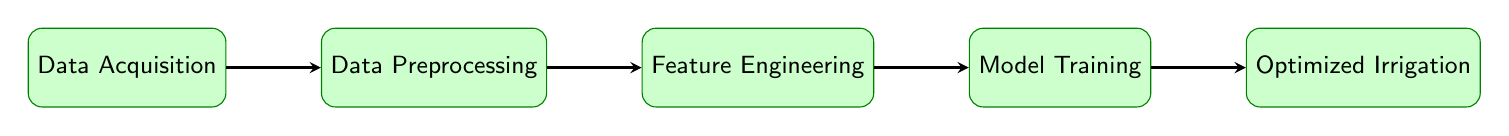
\begin{tikzpicture}[
    node distance=1.5cm and 1.2cm,
    process/.style={
        rectangle, 
        rounded corners=5pt,
        minimum width=1.5cm, 
        minimum height=1cm, 
        align=center, 
        draw=green!50!black,
        fill=green!20,
        font=\small\sffamily
    },
    arrow/.style={thick,->,>=stealth}
]

% Nodes
\node (acq) [process] {Data Acquisition};
\node (pre) [process, right=of acq] {Data Preprocessing};
\node (feat) [process, right=of pre] {Feature Engineering};
\node (train) [process, right=of feat] {Model Training};
\node (opt) [process, right=of train] {Optimized Irrigation};

% Arrows
\draw [arrow] (acq) -- (pre);
\draw [arrow] (pre) -- (feat);
\draw [arrow] (feat) -- (train);
\draw [arrow] (train) -- (opt);

\end{tikzpicture}
\caption{Methodology Flow: From data acquisition to final optimized irrigation.}
\label{fig:methodology_flow}
\end{figure*}
\subsection{Data Acquisition and Preprocessing}
The base of this study is a comprehensive dataset which was acquired from a tomato cultivation experiment, spanning June 29 to September 13 \cite{data}. The data was collected through multi-sensor deployments via the LoRaWAN protocol, at a 10-minute sampling frequency. The sensors and the captured features are given below:
\begin{itemize}
    \item \textbf{Environment sensor:} CO$_2$, air humidity (\%RH), air temp ($^\circ$C) and barometric pressure (hPa).
    \item \textbf{Soil sensor:} soil moisture (\%RH), soil temp ($^\circ$C) and electrical conductivity ($\mu$S/cm). Measurements were taken at a 20cm depth.
    \item \textbf{Water meter:} cumulative water applied per irrigation line (L).
    \item \textbf{Agronomic indicators:} GDD and various heat units.
\end{itemize}

\subsubsection{Preprocessing}
The preprocessing was done as described by the authors in \cite{base}.
\begin{itemize}
    \item \textbf{Data cleaning:} Timestamps were converted to local time, non-informative features were removed, and we also removed all the duplicate entries.
    \item \textbf{Outlier handling for noise and sensor drift:} This was done by statistical detection and a physically based range validation as explained in \cite{base}.
    \item \textbf{Missing data handling:} For shorter gaps, data was filled using forward fill method. For moderate gaps, linear interpolation was used. 10 minute data was synced and aggregated to daily stats (min, max, mean, std). Cumulative water usage was transformed to daily water volume applied.
\end{itemize}

Figures 2 and 3 illustrate the raw sensor data and the unified daily data respectively, which are common for both the baseline and our proposed model.

\begin{figure}[t]
\centerline{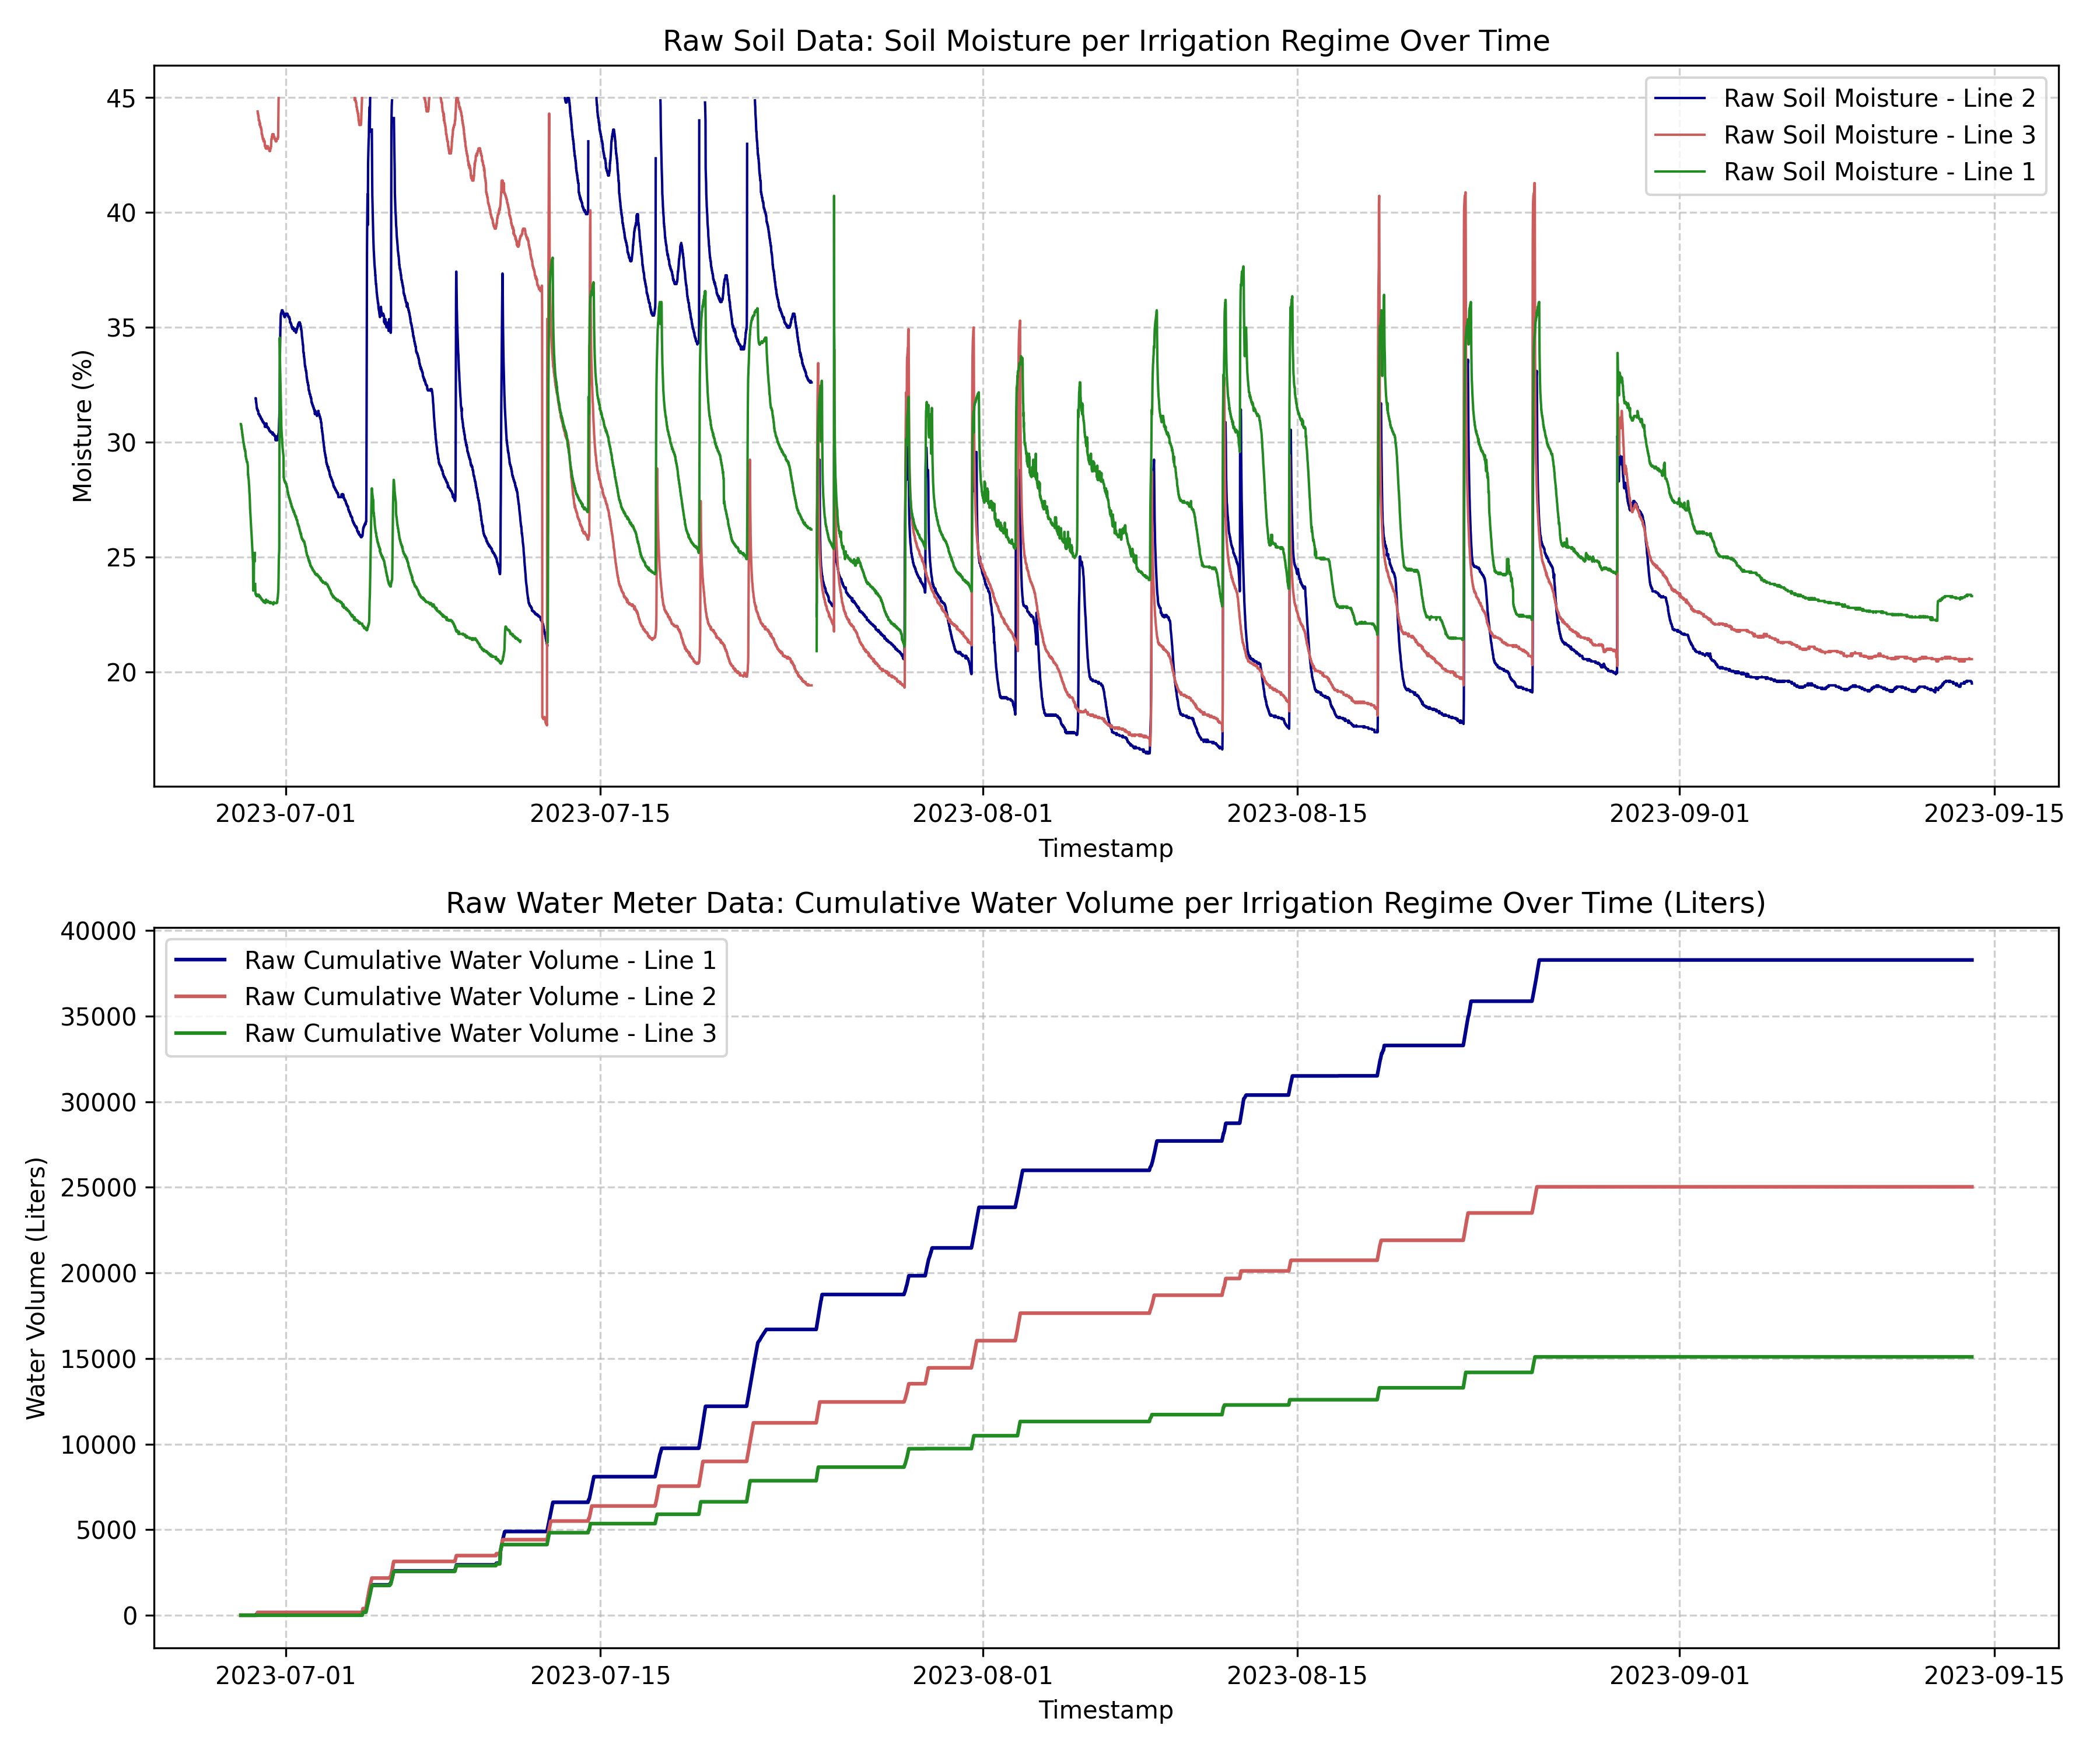
\includegraphics[width=\columnwidth]{Figure_1_Raw_Data.png}}
\caption{Raw IoT sensor data: (a) Soil moisture content per irrigation line, and (b) cumulative water volume per irrigation line (Liters)\cite{base}}
\label{fig1}
\end{figure}

\begin{figure}[t]
\centerline{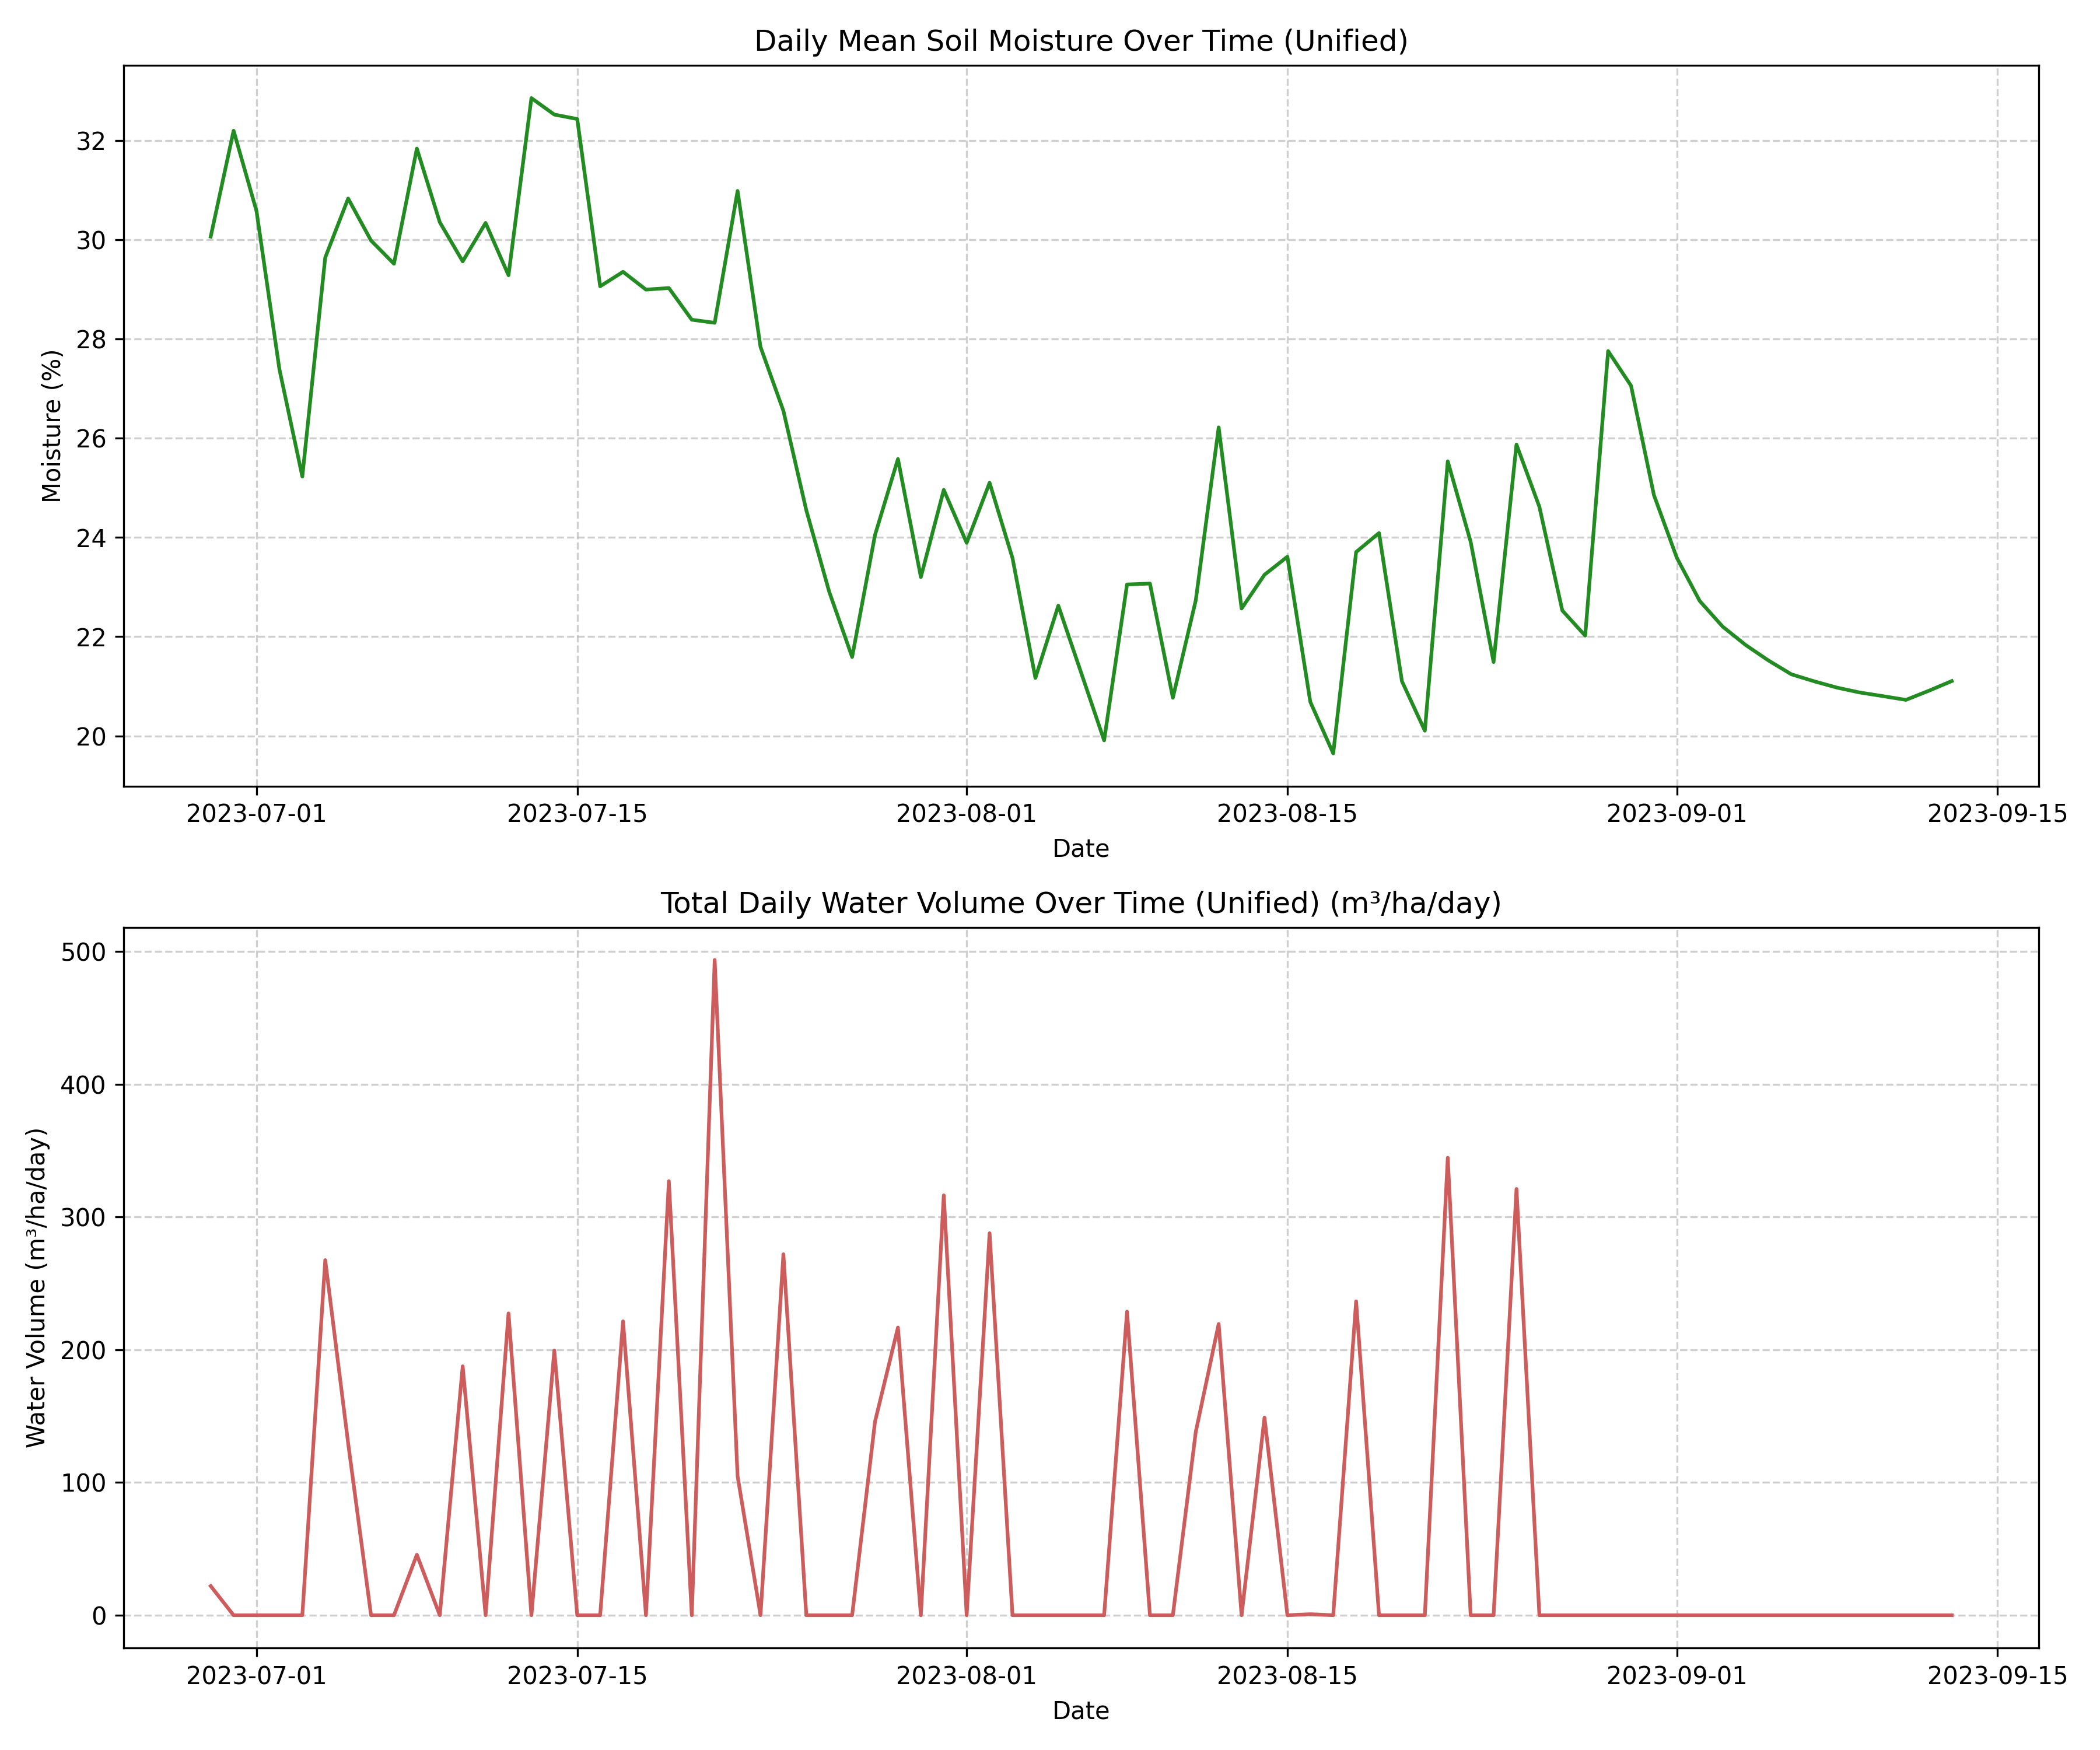
\includegraphics[width=\columnwidth]{Figure_2_Unified_Data.png}}
\caption{Unified daily water and soil parameters: (a) Unified daily mean soil moisture, and (b) unified total daily water volume ($m^{3}/ha/day$)\cite{base}}
\label{fig2}
\end{figure}

\subsection{Feature Engineering}
This was done in 2 phases, one for the engineered features used by the baseline model as mentioned in \cite{base} and the other for the extra features used by our proposed model.

\subsubsection{Baseline}
\begin{itemize}
    \item \textbf{Growing Degree Days (GDD)}
    \begin{equation}
GDD = 
\begin{cases} 
0 & \text{if } T_{avg} \le T_{base} \\ 
T_{avg} - T_{base} & \text{if } T_{base} < T_{avg} < T_{cutoff} \\ 
T_{cutoff} - T_{base} & \text{if } T_{avg} \ge T_{cutoff} 
\end{cases}
\end{equation}
For tomato, $T_{base} = 10^\circ$C and $T_{cutoff} = 32^\circ$C \cite{bctemp}.

    \item \textbf{Electrical Conductivity normalized at $25^\circ$C ($EC_{25}$)}
\end{itemize}
\begin{equation}
EC_{25} = \frac{EC_t}{1 - 0.020346(T_{adj}) + 0.003822(T_{adj})^2 - 0.000555(T_{adj})^3}
\end{equation}
\begin{itemize}
    \item \textbf{Soil Moisture Deficit (SMD):} deviation from predetermined target soil humidity ($25\%$ for tomatoes)
    \begin{equation}
SMD = (T_{SH} - SM_{mean}) \times C_{SM} + EC_{mean} \times C_{EC}
\end{equation}
where $T_{SH}$ is the target SH, and $C_{SM}$ and $C_{EC}$ are weight coefficients valued at 1.5 and 0.15 respectively.
\end{itemize}

Other features are lagged values (1, 3, 7 days), rolling window stats (3, 7 day means and stds). Figure 4 highlights the processed features, 7-day rolling mean and GDD.

\begin{figure}[t]
\centerline{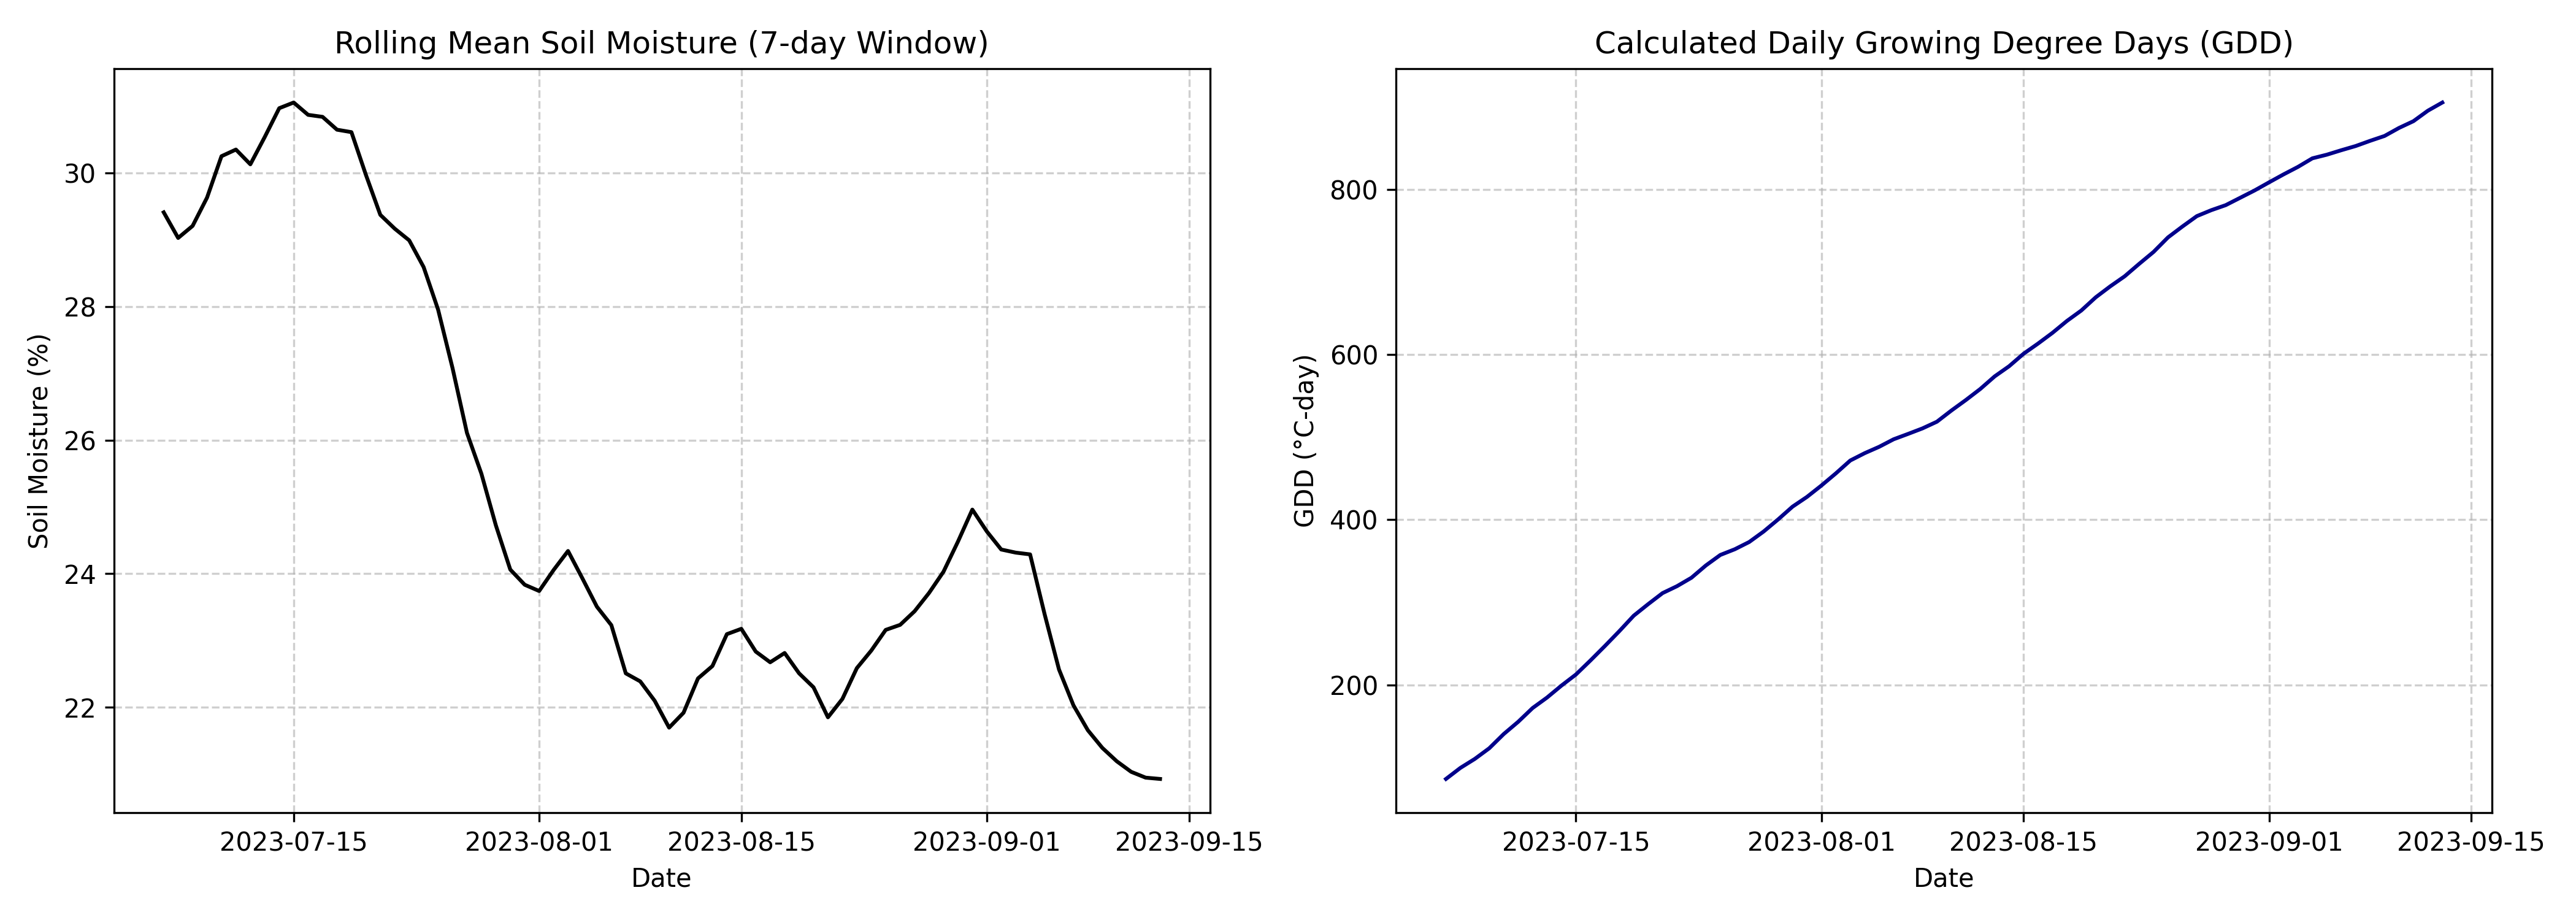
\includegraphics[width=\columnwidth]{Figure_3_Processed_Params.png}}
\caption{Processed agronomic parameters: (a) 7-day rolling mean soil moisture, and (b) calculated daily Growing Degree Days (GDD)\cite{base}}
\label{fig3}
\end{figure}

\subsubsection{Proposed}
\begin{itemize}
    \item \textbf{VPD (Vapor Pressure Deficit) \cite{vpd}:}
    \begin{equation}
    SVP = 0.6108 \times \exp \left( \frac{17.27 \times T_{air\_mean}}{T_{air\_mean} + 237.3} \right)
    \end{equation}
    \begin{equation}
    AVP = SVP \times \left( \frac{RH_{mean}}{100} \right)
    \end{equation}
    \begin{equation}
    VPD = SVP - AVP
    \end{equation}
    
    \item \textbf{Cumulative GDD:} The cumulative sum of the GDD until that day.
    
    \item \textbf{STDR (Soil Temperature Diurnal Range):}
    \begin{equation}
    STDR = T_{soil\_max} - T_{soil\_min}
    \end{equation}
    
    \item \textbf{Heat stress flag:}
    \begin{equation}
    Heat\_Stress = 
    \begin{cases} 
    1 & \text{if } T_{air\_max} \ge 32 \\ 
    0 & \text{if } T_{air\_max} < 32 
    \end{cases}
    \end{equation}
\end{itemize}

\subsection{2 Part XGBoost Model}
\begin{figure}[h]
\centering
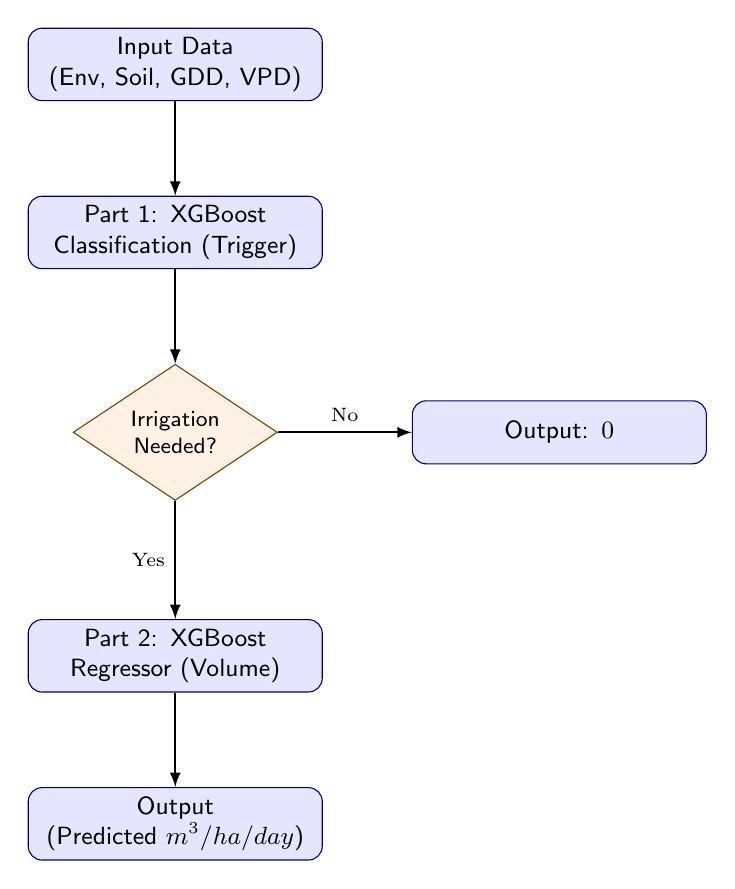
\begin{tikzpicture}[
    node distance=1.2cm,
    block/.style={
        rectangle, 
        rounded corners=5pt, 
        draw=blue!50!black, 
        fill=blue!10, 
        text width=3.5cm, 
        align=center, 
        minimum height=0.8cm,
        font=\small\sffamily
    },
    decision/.style={
        diamond, 
        aspect=1.5,
        draw=orange!50!black, 
        fill=orange!10, 
        text width=1.8cm, 
        align=center, 
        inner sep=0pt,
        font=\footnotesize\sffamily
    },
    line/.style={draw, thick, -latex}
]

\node (input) [block] {Input Data\\(Env, Soil, GDD, VPD)};
\node (clf) [block, below=of input] {Part 1: XGBoost\\Classification (Trigger)};
\node (decide) [decision, below=of clf] {Irrigation\\Needed?};
\node (reg) [block, below=of decide, yshift=-0.3cm] {Part 2: XGBoost\\Regressor (Volume)};
\node (out) [block, below=of reg] {Output\\(Predicted $m^3/ha/day$)};
\node (zero) [block, right=of decide, xshift=0.5cm] {Output: $0$};

\path [line] (input) -- (clf);
\path [line] (clf) -- (decide);
\path [line] (decide) -- node[left, font=\scriptsize] {Yes} (reg);
\path [line] (decide) -- node[above, font=\scriptsize] {No} (zero);
\path [line] (reg) -- (out);

\end{tikzpicture}
\caption{Architecture of the Two-Part XGBoost model, illustrating the conditional execution of the regression layer \cite{base}.}
\label{fig:model_flow}
\end{figure}

The model architecture has been replicated according to the description given in \cite{base} for both the baseline and proposed implementation. The architecture consists of a 2-part XGBoost Model which helps us predict how much water is to be applied to the crops. A flow chart of the architecture is shown in Figure 5 for better understanding.\\
The training data consisted of 40 observations from July 05, 2023 to August 13, 2023. The test set consisted of 31 observations from August 14, 2023 to September 13, 2023 for both the baseline and proposed model.
\begin{enumerate}
    \item \textbf{Classification:} Predicts whether water was applied on a given day (0 or 1).
    \item \textbf{Regression:} If water was applied, predict exact amount of water (m$^3$/ha/day).
\end{enumerate}
The final prediction yields the regressor’s output only if the classifier predicts an irrigation event; otherwise, it outputs zero.

\subsection{Dynamic Irrigation Optimization}
The above model ended up applying a large amount of water and then not applying water in subsequent days. This lead to overuse of water. To optimize the application of water and crop growth, the authors of \cite{base} designed an objective function which the model will aim to minimize.
\begin{equation}
\begin{split}
\text{Objective func} = & (\text{water\_amount} \times 0.05) + \\
& [(\text{water\_amount} - \text{pred\_water\_need})^2 \times 0.005] \\
& + \text{moisture\_penalty}
\end{split}
\end{equation}

\section{Results - Dhyey}
\subsection{Model Performance}
The models were tested on the 31 observations from August 14, 2023 to September 13, 2023. Table \ref{tab_performance}
compares the performance of both the baseline replication \cite{base} and the proposed models. \\
We can observe that the accuracy metrics are not comparable to the results obtained by the authors of \cite{base}. This is because the authors used hyperparameter tuning to improve the choice of hyperparameters to achieve those results.

\begin{table}[htbp]
\caption{Performance Comparison of the Baseline and Proposed models on test set}
\begin{center}
\begin{tabular}{|l|c|c|}
\hline
\textbf{Metric} & \textbf{Baseline Model} & \textbf{Proposed Model} \\
\hline
\multicolumn{3}{|c|}{\textit{Part 1: Classification (Trigger)}} \\
\hline
Accuracy & 0.7419 & \textbf{0.7742} \\
Precision & 0.3636 & \textbf{0.4000} \\
Recall & 0.8000 & 0.8000 \\
F1 Score & 0.5000 & \textbf{0.5333} \\
\hline
\multicolumn{3}{|c|}{\textit{Part 2: Regression (Volumetric m$^3$/ha/day)}} \\
\hline
R$^2$ Score & 0.0241 & \textbf{0.4336} \\
RMSE & 22.6827 & \textbf{17.2801} \\
MAE & 11.4008 & \textbf{8.4648} \\
\hline
\end{tabular}
\label{tab_performance}
\end{center}
\end{table}

We can see that the including the new features in our Proposed model definitely improved the model, showing marginal improvements on the Classifier and significant improvements on the Regressor.\\
Figure 6 shows the actual vs predicted water volumes for our Proposed model.

\begin{figure}[t]
\centerline{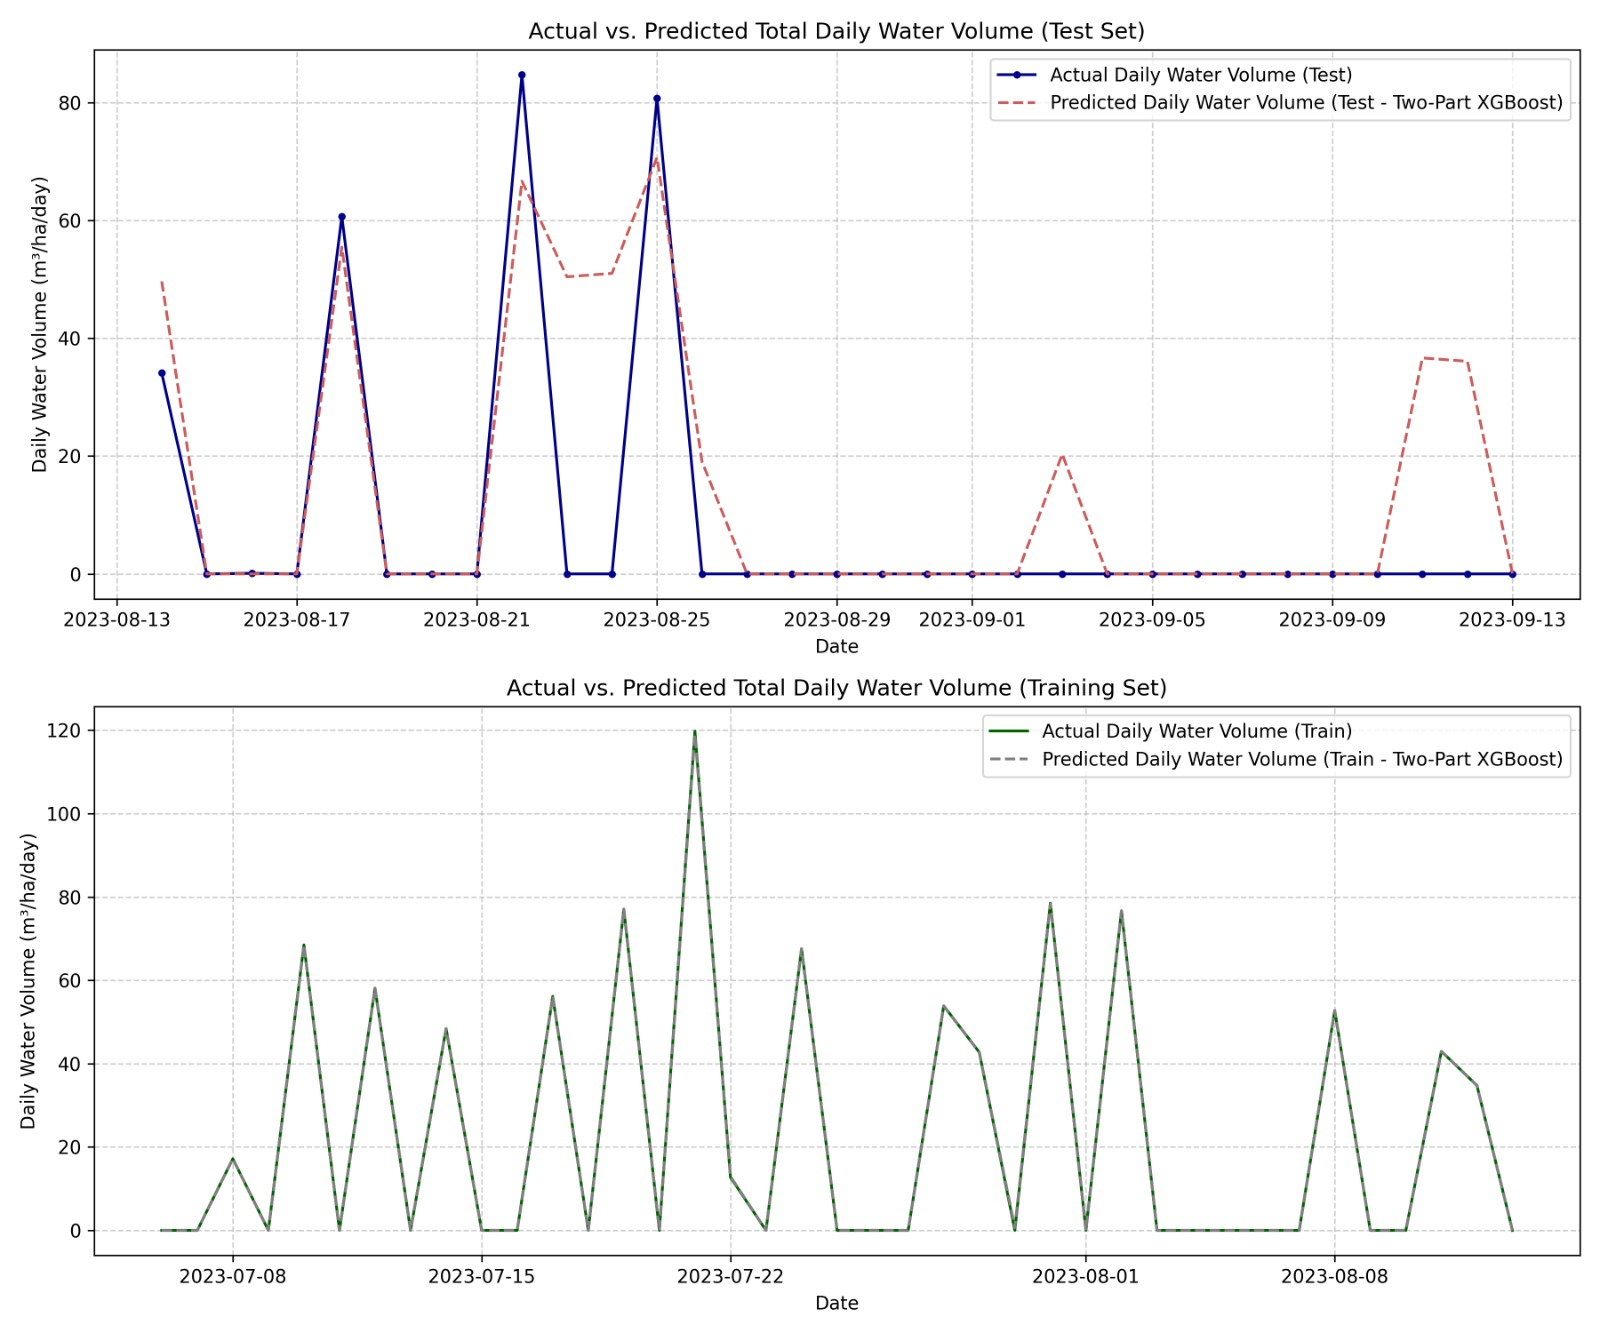
\includegraphics[width=\columnwidth]{Fig4.jpeg}}
\caption{Actual vs Predicted daily water volume \cite{base}}
\label{fig4}
\end{figure}

\subsection{Feature Importance Analysis}
Figure 7 indicates the most important features in our proposed model according to their information gain.

\begin{figure}[t]
\centerline{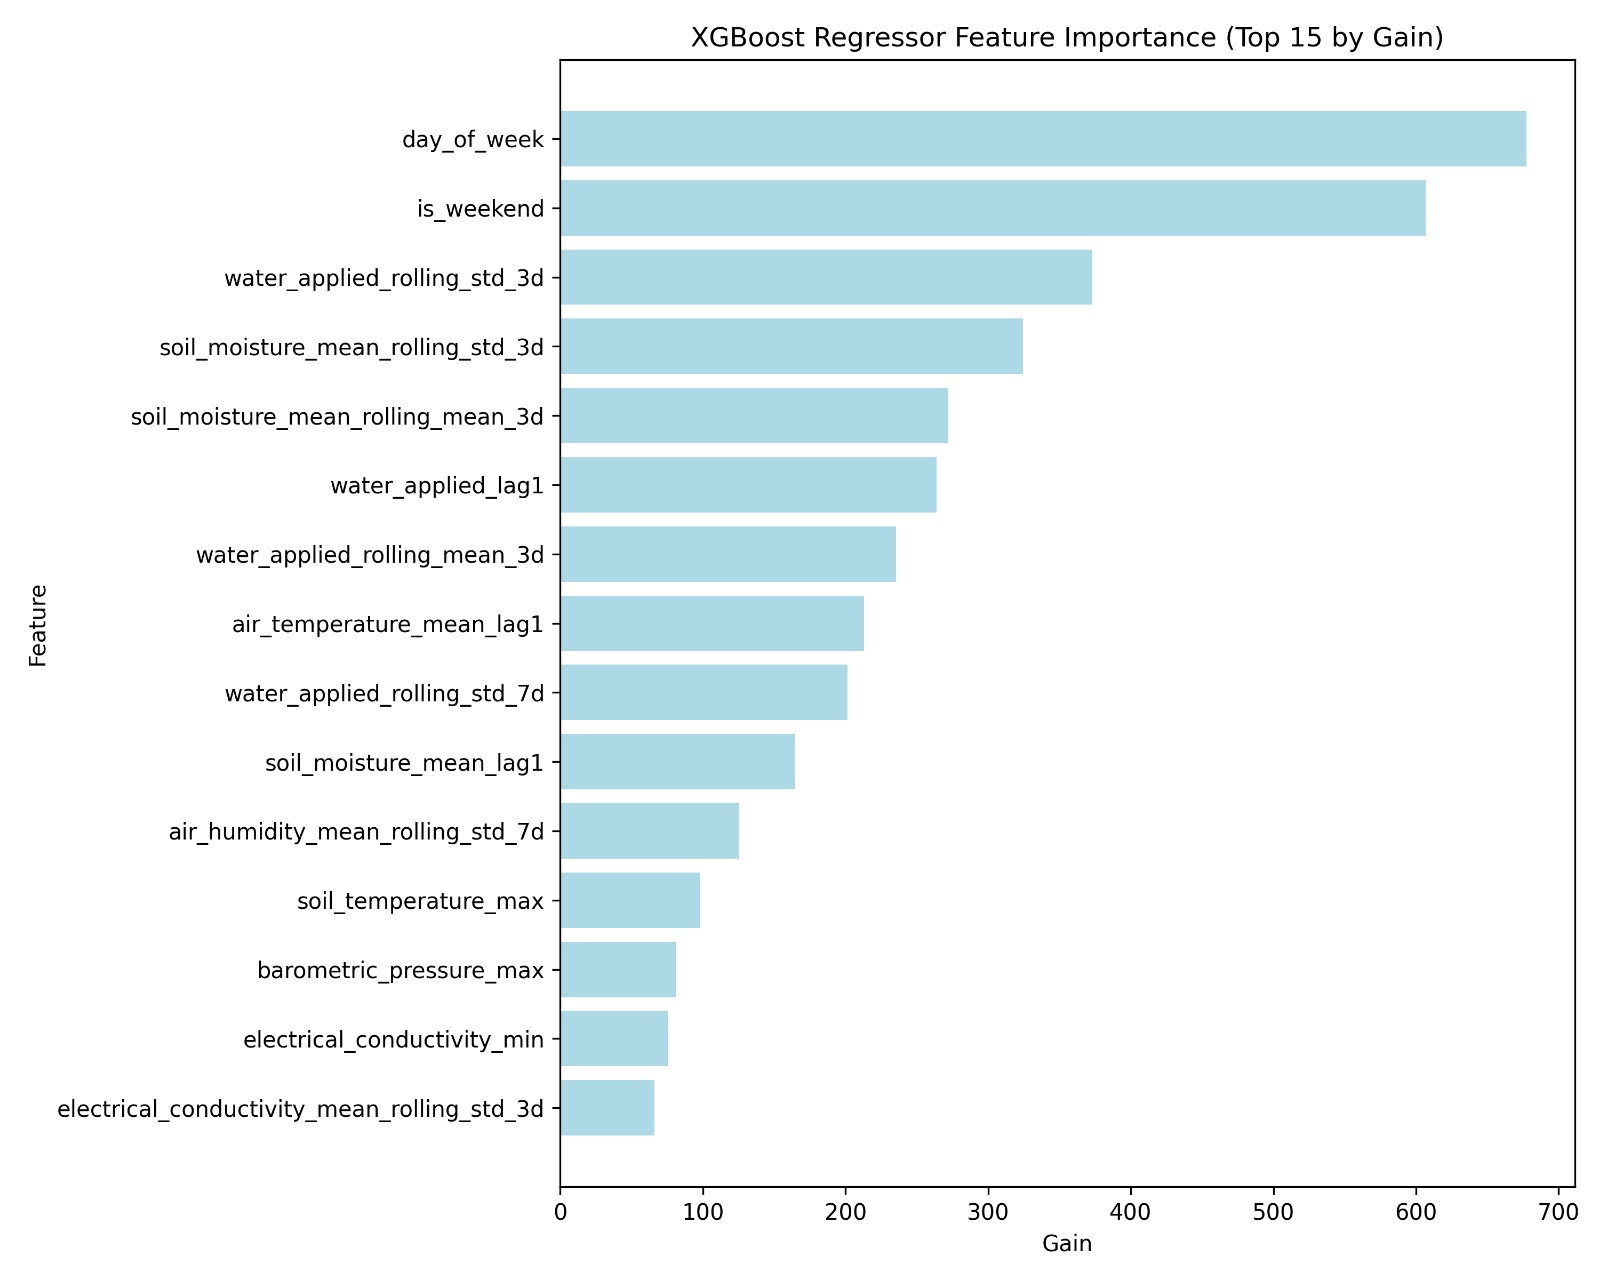
\includegraphics[width=\columnwidth]{Fig5.jpeg}}
\caption{Proposed XGBoost Regressor Feature Importance: High gain seen in engineered features like VPD and cumulative GDD\cite{base}}
\label{fig5}
\end{figure}

\subsection{Dynamic Irrigation Optimization}
Both models were evaluated on the test set, but this time the models were programmed to minimize the objective function to optimize the use of water and crop growth.
The details of the overall water consumption and the simulated savings can be seen in Table \ref{tab_optimization}.

\begin{table}[htbp]
\caption{Dynamic Optimization Simulation Results}
\begin{center}
\begin{tabular}{|l|c|c|}
\hline
\textbf{Metric} & \textbf{Baseline} & \textbf{Proposed} \\
\hline
Total Actual Usage (m$^3$/ha) & 260.23 & 260.23 \\
Model Predicted Usage (m$^3$/ha) & 569.46 & \textbf{455.89} \\
Optimized Applied (m$^3$/ha) & 257.68 & \textbf{222.14} \\
Savings vs. Model Prediction (\%) & 54.75\% & 51.27\% \\
Savings vs. Baseline 10.0 m$^3$/ha (\%) & 16.88\% & \textbf{28.34\%} \\
Avg. Soil Moisture (\%) & 22.63\% & 22.63\% \\
\hline
\end{tabular}
\label{tab_optimization}
\end{center}
\end{table}

We can observe that the proposed model reduced the predicted usage from 569.46 m$^3$/ha to 455.89 m$^3$/ha. Hence the proposed model only applied 222.14 m$^3$/ha while maintaining soil moisture above the 20\% critical threshold. When compared to the static daily irrigation baseline of 10.0 m$^3$/ha, the proposed model achieved a 28.34\% saving, significantly improving on the baseline model's 16.88\% saving. Figure 8 shows the optimal moisture trajectories and targeted irrigation events triggered by the algorithm on our proposed model.

\begin{figure}[t]
\centerline{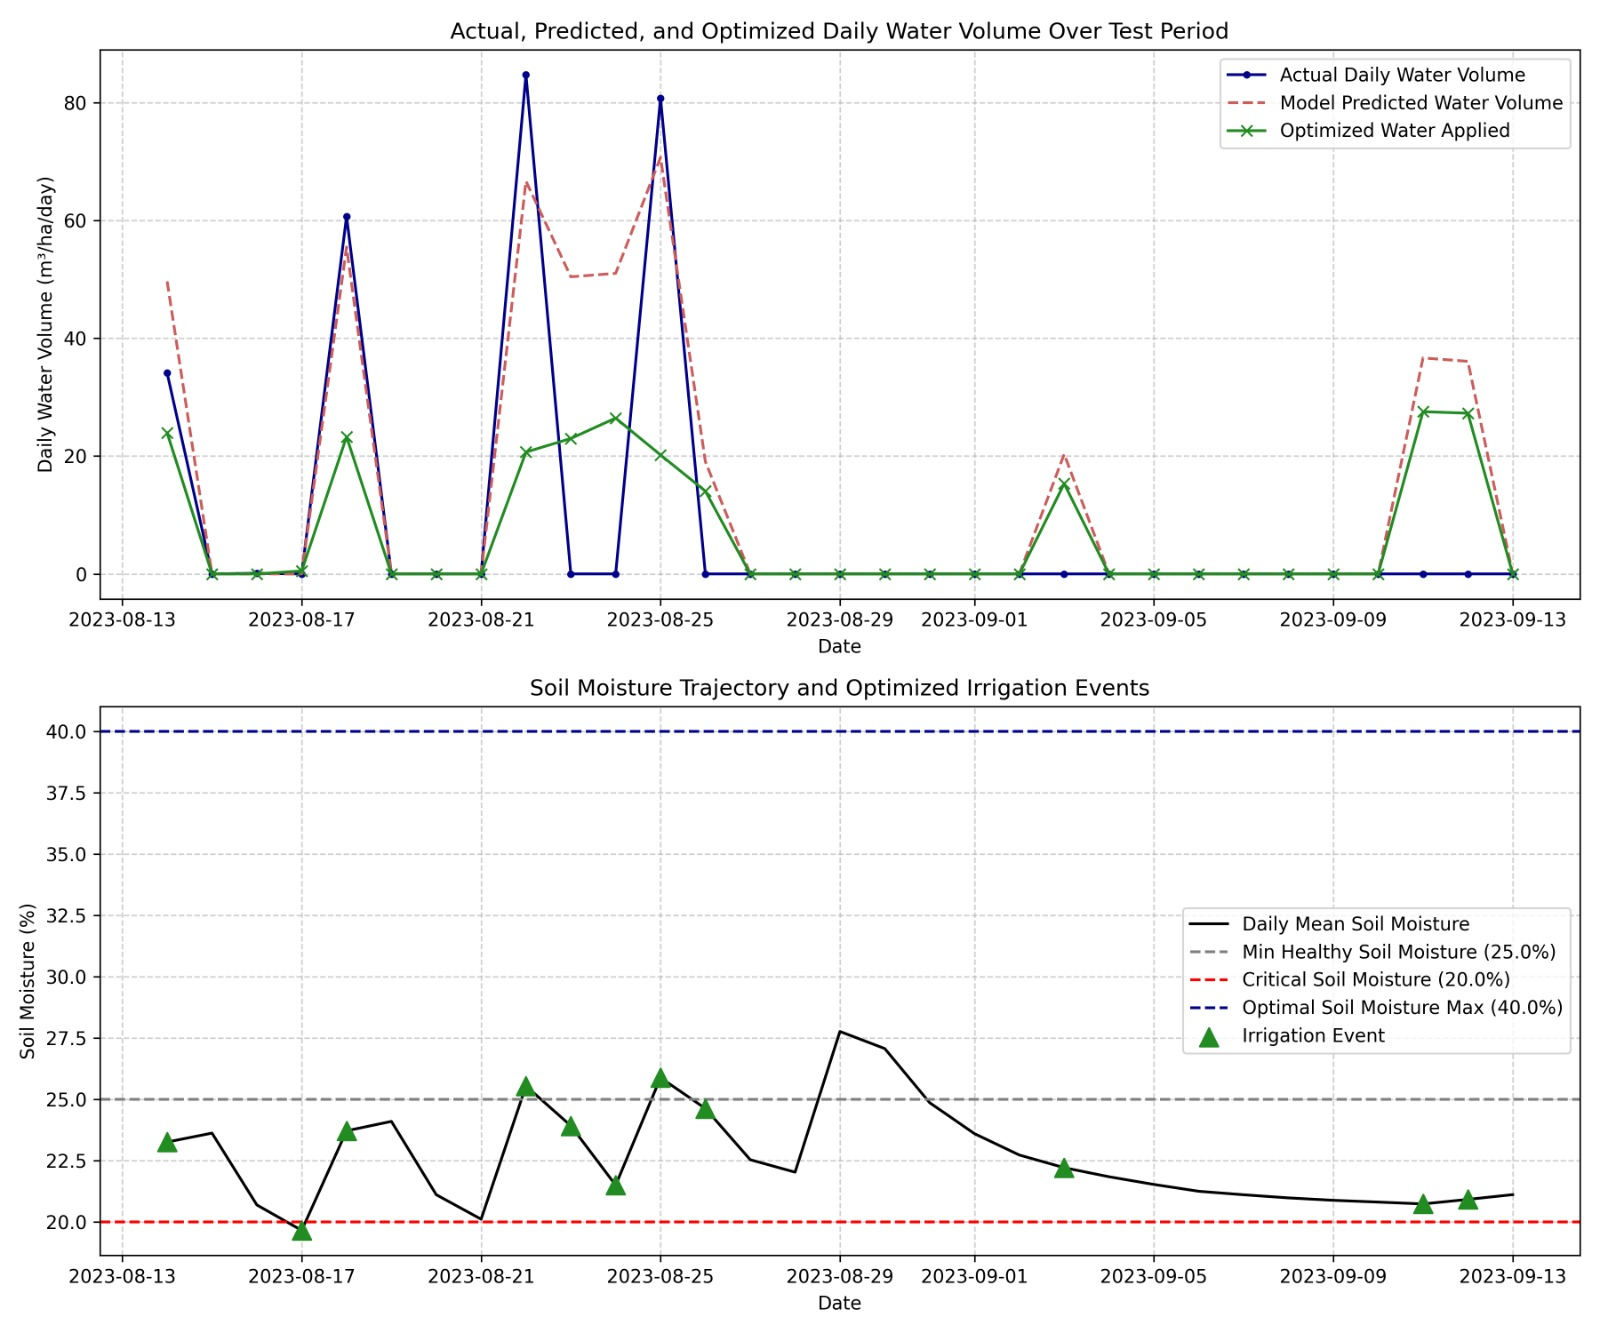
\includegraphics[width=\columnwidth]{Fig6.jpeg}}
\caption{Targeted irrigation events and enhance water savings \cite{base}}
\label{fig5}
\end{figure}

\section{Conclusion - Dhyey}
In this project, we successfully replicated the methodology described in \cite{base}. The results of the implementation yielded an accuracy of 74.19\% instead of 94.76\% stated in \cite{base}. This was because we had not used the hyperparameter tuning which the authors had used. Furthermore, we added new features (i.e. VPD, Cumulative GDD, STDR, etc.) on top of the existing ones using feature engineering in an attempt to improve the existing model. Our proposed model yielded an accuracy of 77.42\% over the existing accuracy of 74.19\% indicating a significant improvement on the model. Then we tried optimizing the use of water by minimizing the objective function described in \cite{base}. The optimization revealed 28.34\% water savings over the 16.88\% savings of the baseline model, compared to a static supply of 10m$^3$ / ha water per day.

\bibliographystyle{IEEEtran}
\bibliography{S0378377421006016,citation-359782665,IJE-10.5829-ije.2026.39.03c.12,citation-398781615, dataset_cit, pericles_exported_citations,dataset,ieee,iot,sensors-v25-i09_20260416,10.3389-fpls.2025.1587869-citation,sensors2, VPD_w,citation-390187813}
\end{document}
